\chapter{}\label{chap12}

\begin{enumerate}
\renewcommand{\labelenumi}{\bf\theenumi.}
\itemsep=5pt

\item ಆರು ಒಂಭತ್ತು ಬಳಸಿ 100 ಬರಿಸಿ 

\item ಐದು 1 ಬಳಸಿ 100 ಬರಿಸಿ

\item ಎಂಟು 8 ಬಳಸಿ 1000 ಬರಿಸಿ. 

\item 0 ಯಿಂದ 9 ರವರೆಗಿನ ಅಂಕಿಗಳನ್ನು ಯಾವುದೇ ಕ್ರಮದಲ್ಲಿ ಒಮ್ಮೆ ಮಾತ್ರ ಬಳಸಿ, $+$ ಮಾತ್ರ ಬಳಸಿ 99 ಬರಿಸಿ. 

\item 5 ಮುರು ಬಳಸಿ 1, 10, 100, 1000 ಬರಿಸಿ. ಯಾವುದೇ ಗಣಿತ ಚಿಹ್ನೆ, ಪ್ರಕ್ರಿಯೆ ಬಳಸಬಹುದು. 

\item ನಾಲ್ಕು 4 ಬಳಸಿ 11 ರಿಂದ 20 ವರೆಗಿನ ಸಂಖ್ಯೆಗಳನ್ನು ಬರಿಸಿ. ಯಾವುದೇ ಗಣಿತ ಚಿಹ್ನೆ, ಪ್ರಕ್ರಿಯೆ ಬಳಸಬಹುದು. 

\item ಒಂದು ಗೆರೆ ಸ್ಥಾನ ಪಲ್ಲಟ ಮಾಡಿ, ಸಮೀಕರನ ಸರಿದೂಗಿಸಿ. $\neq$ ಕೂಡದು. 
\begin{itemize}
\item[(a)] XI $+$ I = X
\item[(b)] C $-$ VI = CV
\item[(c)] IV $-$ II = V
\end{itemize}

\item ಈ ಬೆಂಕಿಕಡ್ಡಿ ಸುರುಳಿ ಗಮನಿಸಿ. 4 ಕಡ್ಡಿ ಸ್ಥಳಾಂತರಿಸಿ, 3ಚೌಕ ಬರಿಸಿ. 
\begin{figure}[H]
\centering
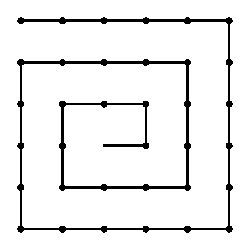
\includegraphics{images/chap12/q8.eps}
\end{figure}

\item 9 ಬೆಂಕಿಕಡ್ಡಿ ಜೋಡಿಸಿ, 10 ಬರಿಸಿ. 

\item ಪ್ರತಿ ಕಡ್ಡಿಯೂ ಬೇರೆ 4ನ್ನು ಸ್ಪರ್ಷಿಸುವಂತೆ 6 ಬೆಂಕಿಕಡ್ಡಿ ಜೋಡಿಸಿ. 

\item 8 ಬೆಂಕಿಕಡ್ಡಿಗಳಿಂದ 2 ಚೌಕ, 4 ತ್ರಿಭುಜದ ರಚಿಸಿ.

\item 4 ಬೆಂಕಿಕಡ್ಡಿಗಳನ್ನು ಈ ರೀತಿ ಜೋಡಿಸಿದೆ. 
\begin{figure}[H]
\centering
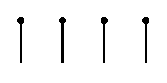
\includegraphics{images/chap12/q12.eps}
\end{figure}


5 ಕಡ್ಡಿ ಸೇರಿಸಿ ಹತ್ತು ಬರಿಸಿ. 

\item 1 2 3 4 5 6 7 9 ಒಂದು ವಿಶಿಷ್ಟ ಸಂಖ್ಯೆ. ಇದನ್ನು 1, 2, 3, 4, 5, 6, 7, 8 ರಿಂದ ಗುಣಿಸಿ. ಗುಣಲಬ್ಧದಲ್ಲಿ ಗುಣಕಗಳ 9ರ ಪೂರಕ ಇರುವುದಿಲ್ಲ. 

ಉದಾ: 
\begin{tabular}[t]{ll}
$1234579\times 1 = 12345679$ & ($9 - 1 = 8$ ಇಲ್ಲ)\\
$1234579\times 2 = 24691358$ & ($9 - 2 = 7$ ಇಲ್ಲ)
\end{tabular}

3 ಮತ್ತು 6 ರಿಂದ ಗುಣಿಸಿದಾಗ ಉತ್ತರ ನೋಡಿ. 

\item ಈ ಗುಣಾಕಾರ ಗಮನಿಸಿ. ಮುಂದಿನ 5ಹಂತ ಬರೆಯಿರಿ. 

\begin{tabular}[t]{ccl}
$32\times 34$ & = & $1~0~88$\\
$332\times 334$ & = & $11~0~88$\\
$3332\times 3334$ & = & $111~0~8888$\\
$33332\times 33334$ & = & $1111~0~88888$\\
\end{tabular}

\item ಈ ಗುಣಾಕಾರ ಗಮನಿಸಿ. ಮುಂದಿನ 5 ಹಂತ ಬರೆಯಿರಿ. 

\begin{tabular}[t]{ccc}
$93\times 94$ & = & $8742$\\
$993\times 994$ & = & $987042$\\
$9993\times 9994$ & = & $99870042$\\
$99993\times 99994$ & = & $9998700042$
\end{tabular}

\item 1 ರಿಂದ 9 ವರೆಗಿನ ಎಲ್ಲ ಅಂಕಿಗಳೂ ಒಮ್ಮೆ ಮಾತ್ರ ಬರುವಂತೆ ಎರಡು ಗುಣಾಕಾರ ರಚಿಸಿ. 

\item ಈ ಗುಣಾಕಾರ ಗಮನಿಸಿ. ಮುಂದಿನ 6 ಹಂತ ಬರೆಯಿರಿ. 

\begin{tabular}[t]{ccl}
$3\times 4$ & = & $12$\\
$33\times 34$ & = & $1122$\\
$333\times 334$ & = & $111222$
\end{tabular}

\item ಈ ಗುಣಾಕಾರಗಳನ್ನು ಗಮನಿಸಿ. 

\begin{tabular}[t]{lllll}
$1\times 2\times 3\times 4 + 1$ & = & $25$ & = & $5^{2}$\\
$1\times 2\times 3\times 4\times 5 + 1$ & = & $121$ & = & $11^{2}$\\
$1\times 2\times 3\times 4\times 5\times 7 + 1$ & = & $841$ & = & $29^{2}$
\end{tabular}

\item ಈ ಆಕೃತಿಯಲ್ಲಿರುವ ಎಲ್ಲಾ ಅಲತೆಯ ಆಯತಗಳೆಷ್ಟು? 
\begin{figure}[H]
\centering
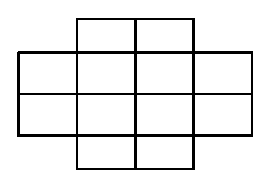
\includegraphics{images/chap12/q19.eps}
\end{figure}

\item 17 ಸೇಬುಗಳನ್ನು ಸಾಲುಗಳಲ್ಲಿ ಜೋಡಿಸಿ 5 ಹಣ್ಣಿನ 2 ಸಾಲು, 4 ಹಣ್ಣಿನ 8 ಸಾಲು ಬರಬೇಕು. 

\item ಈ ಚೌಕದ 4 ಶೃಂಗಗಳನ್ನು ಗಮನಿಸಿ ಪ್ರತಿ ಶೃಂಗವೂ ಸಂಪರ್ಕಿಸುವ 2 ಶೃಂಗಗಳಿಂದ ಸಮಾನ ದೂರದಲ್ಲಿದೆ. ಅದೇ ಸಮತಲದಲ್ಲಿ ಮತ್ತೆ 5 ಬಿಂದುಗಳನ್ನು - ಒಟ್ಟು 9 ಬಿಂದುಗಳು - ಗುರ್ತಿಸಿ. ಪ್ರತಿ ಬಿಂದುವೂ ಬೇರೆ 3 ಬಿಂದುಗಳಿಂದ ಸಮಾನ ದೂರದಲ್ಲಿರಬೇಕು. 
\begin{figure}[H]
\centering
\includegraphics{images/chap12/q21.eps}
\end{figure}

\item ಒಂದು ಘನಾಕಾರದ ರಟ್ಟಿನ ಡಬ್ಬಿಯ ಮೇಲ್ಗಡೆಯ ಭಾಗ ತೆಗೆದು ಹಾಕಿದೆ. ಉಳಿದ ಭಾಗವನ್ನು 4 ಸಮಾನ ವಿಸ್ತೀರ್ಣದ, ಒಂದೇ ರೂಪದ ಆಕೃತಿಗಳಾಗಿ ಕತ್ತರಿಸಿ. 

\item ವೃಕ್ಷಾ ದ್ಹಸ್ತ ಶತೋಚ್ಛ್ರಯಾಚ್ಛತ ಯುಗೇವಾಸೀಂ ಕಪಿಃ ಕೋಽಪ್ರಗಾತ್ ।

ಉತ್ತೀರ್ಯಾಧಪರೋ ದ್ರುತಂ ಶ್ರುತಿ ಪಧೇ ನೋಡ್ಡೀಯಕಿಂಚಿದ್ರುಯಾತ್ ।।

ಜಾತೈವಂ ಸಮತಾತಯೋರ್ಯದಿಗತಾವುಚ್ಚಾಯಮಾನಂ ಕಿಯಾತ್ ।

ವಿದ್ವನ್ ಚೇತ್ ಸುತರಿಶ್ರಸ್ತಿಗಣಿತೇ ಕ್ಷಿಪ್ರಂ ತಸಾಕ್ಷಮೇ ।।

\hfill (ಭಾಸ್ಕರಾಚಾರ್ಯರ `ಲೀಲಾವತೀ'ಯಿಂದ)

{\bf ಅರ್ಥ:}  100 ಮೊಳ ಎತ್ತರವಿರುವ ಒಂದು ಮರದ ಬುಡದಿಂದ 200  ಮೊಳ ದೂರದಲ್ಲಿ ಒಂದು ಭಾವಿ ಇದೆ. ಮರದ ತುದಿಯಲ್ಲಿರುವ ಎರಡು ಕೋತಿಗಳ ಪೈಕಿ ಒಂದು ಮರದಿಂದಿಳಿದು ಭಾವಿ ಹೋಗುತ್ತದೆ. ಇನ್ನೊಂದು ಕೋತಿಯು ಮರದಿ ಮ್ದ ಸ್ವಲ್ಪದೂರ ಮೇಲಕ್ಕೆ ಹಾರಿ, ಭಾವಿಗೆ ನೇರವಾಗಿ ಅಂತರಿಕ್ಷ ಮಾರ್ಗವಾಗಿ ಬರುತ್ತದೆ. ಎರಡು ಕೋತಿಗಳು ಚಲಿಸಿದ ದೂರ ಸಮನಾದರೆ, ಎರಡನೆ ಕೋತಿಯು ಮರದಿಂದ ಎಷ್ಟು ಮೇಲಕ್ಕೆ ಹಾರಿತು ಎಂಬುದನ್ನು ಹೇಳು. 

\item ಇದು ಕೂಡುವ ಲೆಕ್ಕ. ಅಂಕಿಗಳಿಗೆ ಬದಲು ಚಿಹ್ನೆಗಳನ್ನು ಬಳಸಿದೆ. ಒಂ ಚಿಹ್ನೆ ಒಂದೇ ಅಂಕಿಯನ್ನು ಸೂಚಿಸುತ್ತದೆ. ಅಂಕಿಗಳನ್ನು ಕಂಡುಹಿಡಿಯಿರಿ. 
\begin{figure}[H]
\centering
\includegraphics{images/chap12/q24.eps}
\end{figure}


\item ಒಂದು ಚೌಕವನ್ನು 5 ಸಮಾನ ವಿಸ್ತೀರ್ಣವುಳ್ಳ ಭಾಗಗಳಾಗಿ ಕತ್ತರಿಸಬೇಕು. ಭಾಗಗಳ ಆಕಾರ ಒಂದೇ ಇರಬೇಕಿಲ್ಲ. ಎಷ್ಟು ವಿಧಾನಗಳಲ್ಲಿ ಮಾಡಬಹುದು. ಯತ್ನಿಸಿ.  

\item ಯಾತಂ ಹಮ್ಸಕುಲಸ್ಯ ಮೂಲದಶಕಂ ಮೇಘಾಗಮೇ ಮಾನಸಂ ।

ಪ್ರೋಡ್ಡೀಯ ಸ್ಥಲ ಪದ್ಮಿನೀ ವನಮಗಾದಷ್ಟಾಂಶಕೋಽ ಮ್ಭಸ್ತಟಾತ್ ।।

ಬಾಲೇ ಬಾಲ ಮೃಣಾಲ ಶಾಲಿನಿ ಜಲೇ ಕೇಲಿಕ್ರಿಯಾಲಾಲಸಂ ।

ದೃಷ್ಟಂ ಹಂತ ಯುಗತ್ರಯಂಚ ಸಕಾಲಾಂ ಯೂಥಸ್ಯ ಸಂಖ್ಯಾಂವದ ।।

\hfill (ಭಾಸ್ಕರಾಚಾರ್ಯರ ``ಲೀಲಾವತೀ"ಯಿಂದ)


ಅರ್ಥ: ವರ್ಷಾಕಾಲವು ಸಮೀಪಿಸಲಾಗಿ, ಒಂದು ಕೆರೆಯಲ್ಲಿದ್ದ ಹಂಸಗಳ ಪೈಕಿ, ಅವುಗಳ ಸಂಖ್ಯೆಯ ವರ್ಗ ಮೂಲದ ಹತ್ತರಷ್ಟು ಮಾನಸ ಸರೋವರಕ್ಕೆ ತೆರಳಿದುವು. $\dfrac{1}{8}$ ಭಾಗವು ಸ್ಥಳ ಪದ್ಮಿನೀ ವನಕ್ಕೆ ಹೋದುವು. ಉಳಿದ 3ಜೊತೆ ಹಂಸಗಳು ಜಲಕ್ರೀಡೆಯಲ್ಲಿ ಮನಸ್ಸುಳ್ಳವಾಗಿ ಕೆರೆಯಲ್ಲೇ ಇದ್ದುವು. ಹಂಸಗಳ ಒಟ್ಟು ಸಂಖ್ಯೆ ಎಷ್ಟು? 

\item ಈ ಆಕೃತಿಗಳಲ್ಲಿ ಯಾವುದರಲ್ಲಿ ಹೆಚ್ಚು ತ್ರಿಭುಜಗಳಿವೆ? ಎಷ್ಟು ಹೆಚ್ಚು?
\begin{figure}[H]
\centering
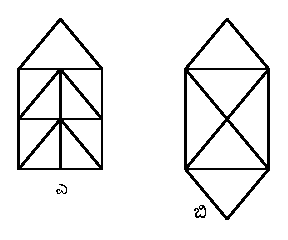
\includegraphics{images/chap12/q27.eps}
\end{figure}

\item ಗಾಂಪರು ಮತ್ತು ಕಳ್ಳರು. 

ಗಾಂಪರ ಮಠದಲ್ಲಿ 64 ಹಸುಗಳಿದ್ದುವು. ಅವುಗಳನ್ನು 8ರ ಗುಂಪು ಮಾಡಿ ಬಯಲಿನಲ್ಲಿ ಕಟ್ಟುತ್ತಿದ್ದರು. ಯಾವ ಮೂಲೆಯಿಂದ ನೊಡಿದರೂ 24 ಹಸುಗಳು ಕಂಡು ಬರುತ್ತಿದ್ದುವು. 
\begin{figure}[H]
\centering

\includegraphics{images/chap12/q28a.eps}
\end{figure}
ಇದು ಗಾಂಪರ ಜೋಡಣೆ.

ಒಟ್ಟು 64


ಒಂದು ದಿನ ಇಬ್ಬರು ಕಳ್ಳರು 8 ಹಸುಗಳೊಂದಿಗೆ ಬಂದರು. ರಾತ್ರಿ ಉಳಿಯಲು ತಮಗೆ, ಹಸುಗಳಿಗೆ ಆಶ್ರಯ ಬೇಡಿದರು. ಹಸುಗಳ ಮುಖ್ಯಸ್ಥ ಮಂಕ ಒಪ್ಪಿದ. ಆದರೆ ಯಾವ ಮೂಲೆಯಿಂದ ನೊಡಿದರೂ 24 ಬರಬೇಕೆಂಬ ಷರತ್ತನ್ನು ಹೇಳಿದ. ಕಳ್ಳರು ಒಪ್ಪಿದರು. ಬೆಳಿಗ್ಗೆ  5 ಗಂಟೆಗೆ ಎದ್ದು ತಮ್ಮ ಹಸುಗಳೊಂದಿಗೆ ಹೋಗುವುದಾಗಿ ಹೇಳಿದರು. 

ಕಳ್ಳರು ಮಾಡಿದ ಜೋಡಣೆ. 
\begin{figure}[H]
\centering
\includegraphics{images/chap12/q28b.eps}
\end{figure}

ಒಟ್ಟು 72


ಬೆಳಿಗ್ಗೆ ಕಳ್ಳರು ತಮ್ಮ ಹಸುಗಳ ಜೊತೆಗೆ ಮಠದ 8 ಹಸುಗಳನ್ನು ಕದ್ದೊಯ್ದರು. ಆದರೆ ಹಸುಗಳ ಗುಂಪನ್ನು ಯಾವ ಮೂಲೆಯಿಂದ ನೋಡಿದರೂ 24 ಕಂಡು ಬಂದುವು. ಹೇಗೆ? 

\item ಒಂದು ಸಂಖ್ಯೆಯ ಎಲ್ಲ ಅಪರವರ್ತನಗಳನ್ನು (ಸಂಖ್ಯೆಯನ್ನು ಹೊರತು ಪಡಿಸಿ) `ತದಿತರ ಭಾಜಕ' (aliquot division) ಎನ್ನುತ್ತಾರೆ. ಎರಡು ಸಂಖ್ಯೆಗಳಲ್ಲಿ ಒಂದರ ತದಿತರ ಭಾಜಕಗಳ ಮೊತ್ತ ಇನ್ನೊಂದು ಸಂಖ್ಯೆಯಾಗಿದ್ದು, ಎರಡನೆ ಸಂಖ್ಯೆಯ ತದಿತರ ಭಾಜಕಗಳ ಮೊತ್ತ ಮೊದಲ ಸಂಖ್ಯೆಯಾದರೆ ಆ ಸಂಖ್ಯೆಗಳು `ಮೈತ್ರಿ ಸಂಖ್ಯೆಗಳು' (amicable numbers). 

ಉದಾ: 1184 ಮತ್ತು 1210

1184ರ ತದಿತರ ಭಾಜಕಗಳು 1, 2, 4, 8, 16, 32, 37, 74, 148, 296, 592

ಇವುಗಳ ಮೊತ್ತ: 1 $+$ 2 $+$ 4 $+$ 8 $+$ 16 $+$ 32 $+$ 37 $+$ 74 $+$ 148 $+$ 296 $+$ 592 = 1210

1210ರ ತದಿತರ ಭಾಜಕಗಳು: 1, 2, 5, 10, 11, 22, 55, 110, 121, 212, 605

ಇವುಗಳ ಮೊತ್ತ 1184 

$\therefore\quad$ 1210, 1184 ಮೈತ್ರಿ ಸಂಖ್ಯೆಗಳು 

ಇವುಗಳ ಬಗ್ಗೆ 11ನೆ ಶತಮಾನದ ಗಣಿತಜ್ಞ ಎಲ್ ಮದ್‌ಷ್ರಿಟಿ EL Madschriti ಪ್ರಸ್ತಾಪಿಸಿದ. 

18ನೆ ಶತಮಾನದ ಆಯ್ಲರ್ 60 ಜೊತೆ ಮೈತ್ರಿ ಸಂಖ್ಯೆಗಳ ಪಟ್ಟಿ ಮಾಡಿದ. 

19ನೆ ಶತಮಾನದಲ್ಲಿ ಪಗಾವಿನಿ ತನ್ನ 16ನೆ ವಯಸ್ಸಿನಲ್ಲಿ 1184, 1210 ಪತ್ತೆ ಮಾಡಿದ. (ಆಯ್ಲರ್ ಬಿಟ್ಟಿದ್ದ). 

ಕೆಲವು ಮೈತ್ರಿ ಸಂಖ್ಯೆಗಳು 

\begin{tabular}[t]{ll}
220, 284 & 6232, 6368\\
2620, 2924 & 10744, 10856\\
5020, 5564 & 17296, 18416
\end{tabular}

\item ರಾಮಾನುಜನ್ ಸಂಖ್ಯೆ  1729. ಎರಡು ಘನಗಳ ಮೊತ್ತವಾಗಿ ಎರಡು ವಿಧಗಳಲ್ಲಿ ನಿರೂಪಿಸಬಹುದಾದ ಅತಿ ಚಿಕ್ಕ ಸಂಖ್ಯೆ  $1^{3} + 12^{3} = 10^{3} + 9^{3} = 1729$

ಇದೇ ಗುಣ ಹೊಂದಿರುವ 1729ಕ್ಕಿಂತ ಅಧಿಕವಾಗಿರುವ ಹಲವಾರು ಸಂಖ್ಯೆಗಳನ್ನು ಪತ್ತೆಹಚ್ಚಲಾಗಿದೆ. 

\begin{tabular}[t]{ll}
$166{3} + 2^{3} = 15^{3} + 9^{3} = 4104$ & ಸಂಖ್ಯಾ ಮಾಂತ್ರಿಕ ಡಿ. ಆರ್. ಕಾಪಶೀಕರ್\\
$24^{3} + 2^{3} = 20^{3} + 18^{3} = 13832$& ರವರು ಇಂತಹ ಸಂಖ್ಯೆಗಳ ಪಟ್ಟಿಯನ್ನೇ\\
$34^{3} + 9^{3} = 33^{3} + 16^{3} = 40033$ & ರಚಿಸಿದ್ದಾರೆ. 
\end{tabular}

ಇದಕ್ಕಿಂತ ವಿಶಿಷ್ಟವೆಂದರೆ 3, 4, 5, 6 ವಿಧಗಳಲ್ಲಿ ಎರಡು ಘನಗಳ ಮೊತ್ತವಾಗಿ ನಿರೂಪಿಸಲ್ಪಡುವ ಸಂಖ್ಯೆಗಳು. ಇದಕ್ಕೆ ಟ್ಯಾಕ್ಸಿ ಕ್ಯಾಬ್ ಸಂಖ್ಯೆ ಎಂದು ಹೆಸರಿದೆ.
\begin{align*}
T_{2} : & 1729 = 10^{3} + 9^{3} = 12^{3} + 1^{3}\\
T_{3} : & 87539319 = 167^{3} + 436^{3} = 228^{3} + 423^{3} = 255^{3} + 414^{3}\\
T_{4} : & 6963472309248 = 2421^{3} + 19083^{3} = 5436^{3} + 10948^{3}\\
& = 1-200^{3} + 18072^{3} = 13322^{3} + 16630^{3}\\
T_{5} : & = 48988659276962496 = 38787^{3} + 365757^{3}\\ 
& = 107839^{3} + 362753^{3} = 221424^{3} + 336588^{3}\\
& = 231518^{3} + 331954^{3}\\
T_{6} : & = 24153319581254312065344= 28906206^{3} + 582162^{3}\\
& = 28894803^{3} + 3064173^{3} = 28657487^{3} + 8519281^{3}\\
& = 27093208^{3} + 16280683^{3} = 265990452^{3} + 17492496^{3}\\
& = 26224366^{3} + 18289922^{3}
\end{align*}

ಈ ರೀತಿ ಆವಿಷ್ಕಾರ ಮುಂದುವರೆಯುತ್ತಲೇ ಇದೆ. 
\end{enumerate}

\smallskip

\begin{center}
\rule{5cm}{1pt}\\[3pt]
{\Large\bfseries ಉತ್ತರಗಳು}\\[-0.1cm]
\rule{5cm}{1pt}
\end{center}

\begin{enumerate}
\item $99 + (99\div 99)$

$99 + 1 = 100$

\item III $-$ II = 100

\item 
\begin{itemize}
\item[(a)] $\dfrac{8888 - 888}{8} = \dfrac{8000}{8} = 1000$
\item[(b)] $\left(8 + \dfrac{8+8}{8}\right)^{\dfrac{8+8+8}{8}} = (10)^{3} = 1000$
\end{itemize}

\item $19+28+30+7+6+5+4 = 99$

\item 
\begin{align*}
\dfrac{3}{3} \times 3^{(3-3)} & = 1\times 1^{\circ} = 1\\
\dfrac{(3\times 3\times 3) + 3}{3} & = \dfrac{30}{3} = 10\\
33\times 3 + \dfrac{3}{3} & = 99 + 1 = 100\\
\left(\dfrac{33-3}{3}\right)^{3} & = \left(\dfrac{30}{3}\right)^{3} = 10^{3} = 1000
\end{align*}

\item 
\begin{itemize}
\item[(a)] $\dfrac{44}{\sqrt{4} + \sqrt{4}} = \dfrac{44}{2+2} = \dfrac{44}{4} = 11$
\item[(b)] $4\times 4 - \sqrt{4} - \sqrt{4} = 16 - 2 - 2 = 12$
\item[(c)] $(4)^{\sqrt{4}} - \sqrt{4} - 4^{\circ} = 16 - 2 - 1 = 13$
\item[(d)] $4 + 4 + 4 + \sqrt{4} = 12 + 2 = 14$
\item[(e)] $4\times 4 - \dfrac{4}{4} = 16 - 1 = 15$
\item[(f)] $4+4+4+4 = 16$
\item[(g)] $4\times 4 + \dfrac{4}{4} = 16 + 1 = 17$
\item[(h)] $4\times 4 + \dfrac{4}{\sqrt{4}} = 16 + \dfrac{4}{2} = 16 + 2 = 18$
\item[(i)] $\dfrac{4}{\sqrt[\cdot]{4}} - \dfrac{4}{4} = \dfrac{4}{\cdot 2} - 1 = 20 - 1 = 19$
\item[(j)] $4\times + \sqrt{4} + \sqrt{4} = 16 + 2 + 2 = 20$
\end{itemize}

\item 
\begin{itemize}
\item[(a)] ಎರಡು ಉತ್ತರಗಳಿವೆ. 
\begin{tabular}[t]{l}
X + I = XI\\
IX + I = X
\end{tabular}
\item[(b)] C $+$ V = CV
\item[(c)] IV $+$ I = V 
\end{itemize}

\item 
\begin{figure}[H]
\centering
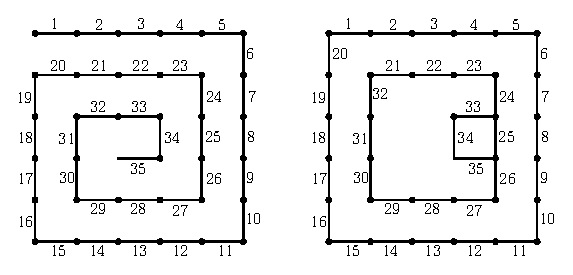
\includegraphics{images/chap12/ans8.eps}
\end{figure}

\item 
\begin{figure}[H]
\centering
\includegraphics{images/chap12/ans9.eps}
\end{figure}

\item 
\begin{figure}[H]
\centering
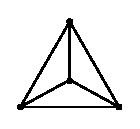
\includegraphics{images/chap12/ans10.eps}
\end{figure}

ಒಂದು [ಪಿರಮಿಡ್ ರಚಿಸಿ (ಅಂಟು ಹಾಕಿ ಜೋಡಿಸಿ)

\item 
\begin{figure}[H]
\centering
\includegraphics{images/chap12/ans11.eps}
\end{figure}

\item 
\begin{figure}[H]
\centering
\includegraphics{images/chap12/ans12.eps}
\end{figure}

\item 
\begin{tabular}[t]{llll}
$12345679\times 4$ & = & $49382716$ & ($9-4 = 5$ ಇಲ್ಲ)\\
$12345679\times 5$ & = & $61728395$ & ($9-5 = 4$ ಇಲ್ಲ)\\
$12345679\times 7$ & = & $86219753$ & ($9-7 = 2$ ಇಲ್ಲ)\\
$12345679\times 8$ & = & $98765432$ & ($9-8 = 1$ ಇಲ್ಲ)
\end{tabular}
\begin{align*}
12345679\times 3 & = 037~037~037\\
12345679\times 6 & = 074~074~074\\ 
\end{align*}

\item 
\begin{tabular}[t]{ccl}
$333332\times 333334$ & = & $1111~0~888888$\\
$333~3332\times 333~3334$ & = & $11111~0~8888888$\\
$333~333~32\times 333~333~34$ & = & $111~111~0~8888~8888$\\
$333~333~332\times 333~333~334$ & = & $111~1111~0~888~888~888$\\
$333~333~3332\times 333~3333~334$ & = & $1111~1111~0~888~888~888$\\
\end{tabular}

\item 
\begin{tabular}[t]{ccc}
$999993\times 99999~4$ & = & $9999~87~0000~42$\\
$999~9993\times 999~999~4$ & = & $99999~87~00000~42$\\
$999~999~93\times 999~999~94$ & = & $999~999~87~000000~42$\\
$999~999~993\times 999~999~994$ & = & $999~9999~87~000~000~42$\\
$999~999~9993\times 999~999~9994$ & = & $999~99999~87~0000~0000~42$
\end{tabular}

\item 
\begin{align*}
27\times 198 & = 5346\\
39\times 186 & = 7254
\end{align*}

\item 
\begin{tabular}[t]{ccc}
$3333\times 3334$ & = & $1111~2222$\\
$33333\times 33334$ & = & $11111~22222$\\
$33~33~33\times 333~334$ & = & $111~111~222~222$\\
$333~333~3\times 333~3334$ & = & $111~1111~222~222~2$\\
$333~333~33\times 333~333~34$ & = & $1111~1111~2222~2222$\\
$333~333~333\times 333~333~334$ & = & $111~111~111~222~222~222$\\
\end{tabular}

\item ಉತ್ತರದ ಅಗತ್ಯವಿಲ್ಲ 

\item 51 ಆಯತಗಳು 

\item 
\begin{figure}[H]
\centering

\includegraphics{images/chap12/ans20.eps}
\end{figure}
\begin{tabular}[t]{ll}
4 ಅಡ್ಡ ಸಾಲು & \\
4 ಕಂಭ ಸಾಲು & 8 ಸಾಲುಗಳು (4 ಹಣ್ಣು)\\[0.2cm]
2 ಕರ್ಣ ಸಾಲು & (5 ಹಣ್ಣು)
\end{tabular}

\item 
\begin{figure}[H]
\centering
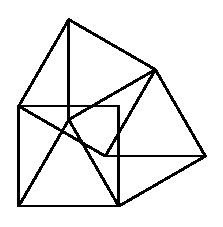
\includegraphics{images/chap12/ans21.eps}
\end{figure}

\item 
\begin{figure}[H]
\centering
\includegraphics{images/chap12/ans22a.eps}
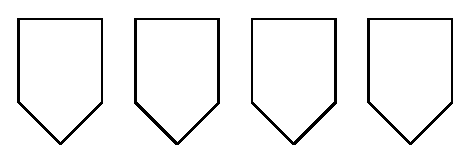
\includegraphics{images/chap12/ans22b.eps}
\end{figure}

\item 
\begin{figure}[H]
\centering
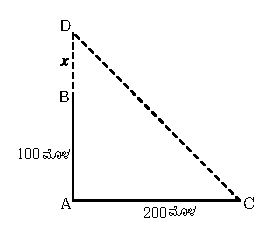
\includegraphics{images/chap12/ans23.eps}
\end{figure}

AB =  ಮರ 100 ಮೊಳ, C ಭಾವಿ, AC = 200

BA $+$ AC ಮೊದಲನೆ ಕೋತಿಯ ಪಥ =100 $+$ 200

BD $+$ DC ಎರಡನೆ ಕೋತಿ ಪಥ. BD = x ಇರಲಿ 
\begin{align*}
CD^{2} & = (x + 100)^{2} + 200^{2}\\
(x+CD) & = BA + AC = 300 \quad\therefore~ CD = 300 - x\\
(300 - x)^{2} & = (x + 100)^{2} + 200^{2}\\
90000 - 600x + x^{2} & = x^{2} + 200x + 10000 + 40000\\
800x & = 90000 - 10000 - 40000\\
800x & = 4000\\
x & = 50 ~\text{ ಮೊಳ}
\end{align*}

\item ಇದನ್ನು ತರ್ಕ ಹಾಗು ತಪ್ಪು-ಒಪ್ಪು ವಿಧಾನದಿಂದ ಬಿಡಿಸಬಹುದು. 0 ಚಿಹ್ನೆಗೆ 1 ಅಥವಾ 2 ಮಾತ್ರ ಬರಬಹುದು. ಹೆಚ್ಚಾದರೆ ಅವುಗಳ ಮೊತ್ತ ಹಿಂದಿನ ದಶಕ ಸೇರಿ, ಉತ್ತರ 4 ಅಂಕಿಯಾಗುತ್ತೆ. $\otimes$ ಚಿಹ್ನೆಗೆ 8 ಅಥವಾ 9 ಇರಬಹುದು. 9 ಇದ್ದರೆ ಮೊತ್ತ 27 ಅಂದರೆ $\ominus$ಯು 7 ಆಗುತ್ತದೆ. 2ನೆ ಸಾಲಿನಲ್ಲಿ ಮೊತ್ತ (2 ದಶಕ ಇರುವುದರಿಂದ) 5 ಬರಬೇಕು ಸಾಧ್ಯವಿಲ್ಲ. $\otimes$ ಚಿಹ್ನೆ 8 ಇದ್ದರೆ ಮೊತ್ತ 24. ಅಂದರೆ $\ominus$ಗೆ 4 ಇರಬೇಕು. ಇದು ಸಾಧ್ಯವಾಗಲು $\ominus$ 4 ಮೊತ್ತ 12. ದಶಕ 2 ಒಟ್ಟು 14 ಆಗುತ್ತದೆ. 

೦ ಚಿಹ್ನೆಗೆ 1 ಇದ್ದರೆ, 1 $+$ 1 $+$ 1 ದಶಕ 1 ಕೂಡಿಸಿದರೆ 4. 

$\therefore\quad$ ಉತ್ತರ
\begin{tabular}[t]{lll}
1 & 4 & 8\\
1 & 4 & 8\\
1 & 4 & 8\\
\hline
4 & 4 & 4\\
\end{tabular}

\item
\begin{figure}[H]
\centering
\includegraphics{images/chap12/ans25a.eps}
\end{figure} 

\begin{figure}[H]
\centering
\includegraphics{images/chap12/ans25b.eps}
\end{figure} 


\item ಹಂಸಗಳ ಸಂಖ್ಯೆ $x$ ಇರಲಿ 

\begin{tabular}[t]{ll}
$10 \sqrt{x}$ & ಮಾನಸ ಸರೋವರಕ್ಕೆ \\
$\dfrac{1}{8} x$ & ಸ್ಥಳ ಪದ್ಮಿನೀ ವನಕ್ಕೆ \\
$3$ಜೊತೆ= $6$ & ಕೆರೆಯಲ್ಲಿ
\end{tabular}

ಒಟ್ಟು $10\sqrt{x} + \dfrac{1}{8}x + 6 = x$

8 ರಿಂದ ಗುಣಿಸಿ $80\sqrt{x} + x + 48 = 8x$

$$80\sqrt{x} = (7x - 48)$$

ವರ್ಗಣೆ ಮಾಡಿ $6400x = 49x^{2} - 672x + 2304$
\begin{align*}
49x^{2} - 7072x + 2304 & = 0\\
(x - 144) (49x - 16) & = 0
\end{align*}
 
 $x = 144$ ಅಥವಾ $\dfrac{16}{49}$ ಭಿನ್ನರಾಶಿ ಹಂಸ ಸಾಧ್ಯವಿಲ್ಲ. 
 
 $\therefore\quad$ ಹಂಸಗಳು 144

\item `ಎ' ಯಲ್ಲಿ 11 ತ್ರಿಭುಜಗಳಿವೆ. 

`ಬಿ' ಯಲ್ಲಿ 10 ತ್ರಿಭುಜಗಳಿವೆ. 

`ಎ' ಯಲ್ಲಿ ಹೆಚ್ಚು ತ್ರಿಭುಜಗಳು 

\item ಕಳ್ಳರು ಹೋಗುವ ಮುನ್ನ ಮಾಡಿದ ಜೋಡಣೆ 
\begin{figure}[H]
\centering
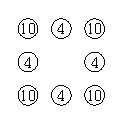
\includegraphics{images/chap12/ans28.eps}
\end{figure} 

ಒಟ್ಟು 56

\item ಉತ್ತರದ ಅಗತ್ಯವಿಲ್ಲ 

\item ಉತ್ತರದ ಅಗತ್ಯವಿಲ್ಲ 
\end{enumerate}
